% Options for packages loaded elsewhere
\PassOptionsToPackage{unicode}{hyperref}
\PassOptionsToPackage{hyphens}{url}
%
\documentclass[
]{article}
\usepackage{lmodern}
\usepackage{amssymb,amsmath}
\usepackage{ifxetex,ifluatex}
\ifnum 0\ifxetex 1\fi\ifluatex 1\fi=0 % if pdftex
  \usepackage[T1]{fontenc}
  \usepackage[utf8]{inputenc}
  \usepackage{textcomp} % provide euro and other symbols
\else % if luatex or xetex
  \usepackage{unicode-math}
  \defaultfontfeatures{Scale=MatchLowercase}
  \defaultfontfeatures[\rmfamily]{Ligatures=TeX,Scale=1}
\fi
% Use upquote if available, for straight quotes in verbatim environments
\IfFileExists{upquote.sty}{\usepackage{upquote}}{}
\IfFileExists{microtype.sty}{% use microtype if available
  \usepackage[]{microtype}
  \UseMicrotypeSet[protrusion]{basicmath} % disable protrusion for tt fonts
}{}
\makeatletter
\@ifundefined{KOMAClassName}{% if non-KOMA class
  \IfFileExists{parskip.sty}{%
    \usepackage{parskip}
  }{% else
    \setlength{\parindent}{0pt}
    \setlength{\parskip}{6pt plus 2pt minus 1pt}}
}{% if KOMA class
  \KOMAoptions{parskip=half}}
\makeatother
\usepackage{xcolor}
\IfFileExists{xurl.sty}{\usepackage{xurl}}{} % add URL line breaks if available
\IfFileExists{bookmark.sty}{\usepackage{bookmark}}{\usepackage{hyperref}}
\hypersetup{
  hidelinks,
  pdfcreator={LaTeX via pandoc}}
\urlstyle{same} % disable monospaced font for URLs
\usepackage{graphicx,grffile}
\makeatletter
\def\maxwidth{\ifdim\Gin@nat@width>\linewidth\linewidth\else\Gin@nat@width\fi}
\def\maxheight{\ifdim\Gin@nat@height>\textheight\textheight\else\Gin@nat@height\fi}
\makeatother
% Scale images if necessary, so that they will not overflow the page
% margins by default, and it is still possible to overwrite the defaults
% using explicit options in \includegraphics[width, height, ...]{}
\setkeys{Gin}{width=\maxwidth,height=\maxheight,keepaspectratio}
% Set default figure placement to htbp
\makeatletter
\def\fps@figure{htbp}
\makeatother
\setlength{\emergencystretch}{3em} % prevent overfull lines
\providecommand{\tightlist}{%
  \setlength{\itemsep}{0pt}\setlength{\parskip}{0pt}}
\setcounter{secnumdepth}{-\maxdimen} % remove section numbering

\date{}

\begin{document}

\hypertarget{header-n0}{%
\subsubsection{Compute rotation around the hinge between the frame and
the steer}\label{header-n0}}

\hypertarget{header-n3}{%
\paragraph{Get axis of rotation}\label{header-n3}}

We computed the axis of rotation in the callibration trial using a
least-squares approach {[}Ehrig2007{]}. We can compute the rotation of
the steer in the coordinate system of the frame \(R^{steer}_{frame}\)
from the orientation of the frame in the world \(R^{frame}_{world}\) and
of the steer in the world \(R^{steer}_{world}\). These orientation of
the world are based on the sensor fusion in Xsens. (Note: we attached
one sensor the the frame of the bike and one sensor to the steer of the
bike. We assume that all rotation occurs around a hinge representing the
stem of the bike)

\[R^{steer}_{frame} = R^{frame^T}_{world} * R^{steer}_{world}\]

Hence we can compute the function axis in the steer (\(\eta_{steer}\))
and in the frame (\(\eta_{steer}\)) by solving this equation in a
least-squares sense (we have n-frames for \(R^{frame}_{steer}\) ). We
solved the least-squares problem using a singular value decomposition in
matlab (using function svd).

\[\eta_{frame} = R^{frame}_{steer} \eta_{steer}\]

In the next step we want to compute the rotation around this axis.
Therefore, we adapted the coordinate system (\(R\)) of the frame such
that the x-axis aligns with \(\eta_{frame}\).

\[z = n_{frame} \times \begin{bmatrix} 0 & 1 & 0 \end{bmatrix}\]

\[y = z \times n_{frame}\]

\[R = \begin{bmatrix} n_{frame} & y & z \end{bmatrix}\]

As a result we can compute the rotation around the axis of rotation in a
rotation matrix (\(R_{axis}\)) and convert it to euler angles
(\(\theta_{stuurRot}\))

\[R_{axis} = R*R^{steer}_{frame}\]

\[\theta_{stuurRot} = rotm2eul(R_{axis})\]

\hypertarget{header-n15}{%
\paragraph{Result}\label{header-n15}}

This works well in most cases. In figure 1 you can see that the error on
equations 2 is low during the callibration, there is only movement along
the stem of the bike during the callibration trial. Futhermore, we
steering angle looks fine during the whole movement.

In some trials, mainly with the normal bike, we see also rotation around
the y and z axis, which we don't expect. On the one hand, this might be
related to different sensor placement and the stem of the bike. On the
other hand, the rotation is too large to be explained by a loose stem of
the bike...

\begin{figure}
\centering
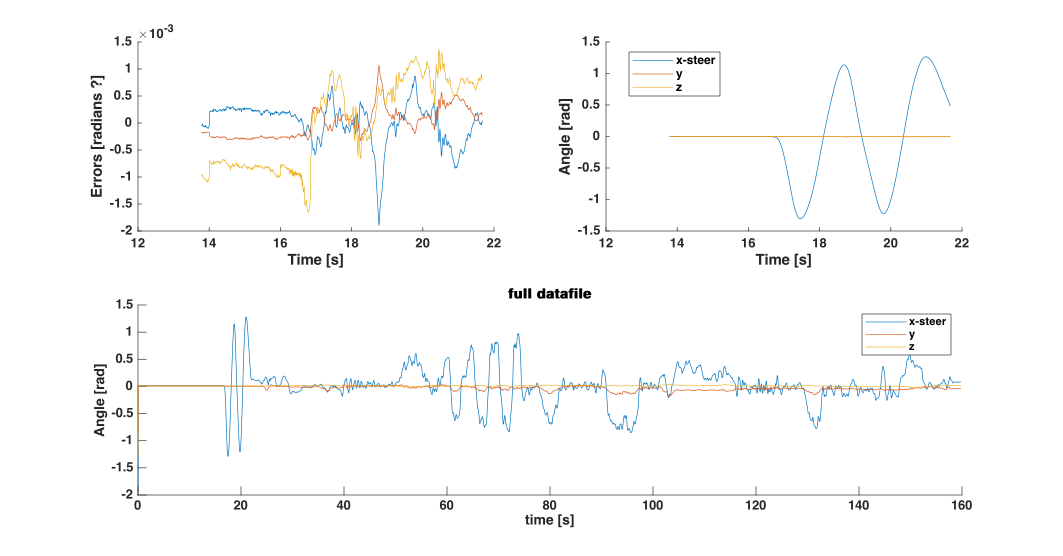
\includegraphics{C:/Users/u0088756/Documents/Teaching/MasterThesis/Anouck_Theresa/Software/Manuals/RotationStem/figs/Callibration_succesfull.svg}
\caption{}
\end{figure}

Figure 1: ...

\begin{figure}
\centering
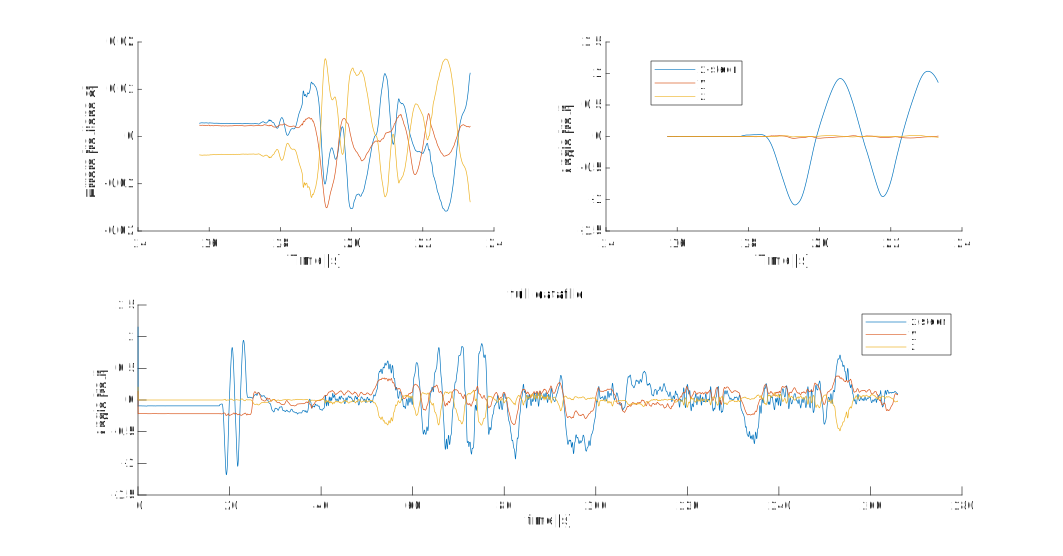
\includegraphics{C:/Users/u0088756/Documents/Teaching/MasterThesis/Anouck_Theresa/Software/Manuals/RotationStem/figs/Callibration_NotSuccesfull.svg}
\caption{}
\end{figure}

\emph{Figure 2}

\hypertarget{header-n25}{%
\paragraph{Batch processing in matlab}\label{header-n25}}

You have to run the script \emph{GetRotationAxisSteer\_Subjects.m} to:

\begin{itemize}
\item
  Compute the axis of rotation in each subjects with the normal bike and
  the classic bike
\item
  Compute the steering angle in all subjects and trials.
\end{itemize}

These scripts mainly rely on the functions

\begin{itemize}
\item
  getCallibrationPhase.m automatically detect the callibration phase
\item
  GetHingeAxis.m to compute the rotation axis
\item
  GetAngleSteer.m to compute the steering angle
\item
  InterpolateRotMatrices.m to interpolate the orienations of the sensors
  when frames are missing (not very common). We first convert to
  rotation matrices to euler angles, interpolate the euler angles and
  convert to rotation matrices again.
\end{itemize}

\hypertarget{header-n43}{%
\subsubsection{References}\label{header-n43}}

Ehrig2007: A survey of formal methods for determining functional joint
axes

\end{document}
